\documentclass[11pt,twoside]{SEEELab_V1}

% ---- Metadata ----
\labtitle{Experiment 1 --- DC Motor / PID Control}
\labsubtitle{} % leave empty to hide line
\labauthor{Farhan Aizuddin}
\labdate{September 18, 2025}
\coursecode{EEM441}
\semester{Semester I (2025/2026)}
\lablogo{Figures/Logo_USM_SEEE.png} % (optional)

\graphicspath{{Figures/}}

\begin{document}
\makelabtitle
\makemargintoc

\section{Introduction}
This experiment covers the basics of DC motor and PID control.

\section{Methodology}
\subsection{Open-Loop Speed Control of a DC Motor}
\begin{enumerate}
  \item Switch on supply and measure all constant voltages and calibrate variable voltages in terms of voltages and angles in degrees.
  \item Disconnect all cable wires from the hardware module.
  \item Make circuitry as shown in Fig.~\ref{fig:openloop} for the implementation of open-loop speed control of a DC motor.
  \item Connect Output A of the motor plant to channel 2 of the oscilloscope.
\end{enumerate}

\begin{figure}[ht]
  \centering
  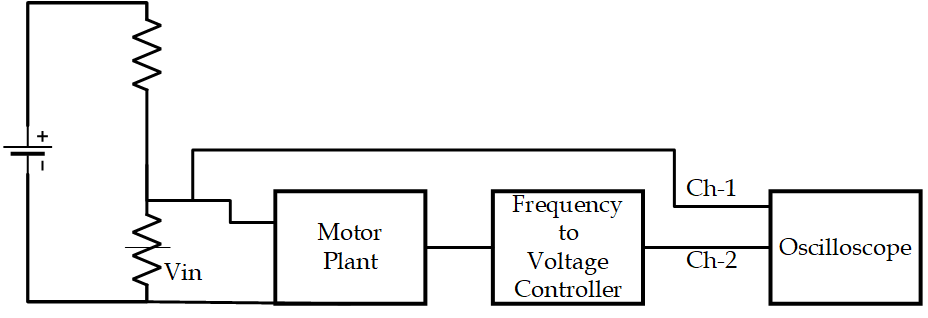
\includegraphics[width=0.9\linewidth]{OpenLoopMotorControl.png}
  \caption{Open-loop speed control setup.\label{fig:openloop}}
\end{figure}

\appendix
\section{Appendix}
Additional reference material.

\end{document}
